              %******************************************%
              %                                          %
              % Modello di tesi di laurea o di dottorato %
              %            di Lorenzo Pantieri           %
              %                                          %
              %                © 2013-2017               %
              %                                          %
              %******************************************%
       

% I seguenti commenti speciali impostano:
% 1. utf8 come codifica di input,
% 2. PDFLaTeX come motore di composizione;
% 3. Tesi.tex come documento principale;
% 4. il controllo ortografico italiano per l'editor.

% !TEX encoding = UTF-8 Unicode
% !TEX TS-program = pdflatex
% !TEX root = Tesi.tex
% !TEX spellcheck = it-IT

\documentclass[11pt,%                      % corpo del font principale
               a4paper,%                   % carta A4
               twoside,openright,%         % fronte-retro
%              oneside,openany,%           % solo fronte
               titlepage,%                 % frontespizio
               headinclude,,footinclude,%  % testatina e piede di pagina
               BCOR5mm,%                   % rilegatura di 5 mm
               cleardoublepage=empty,%     % pagine vuote senza testatina e piede di pagina
               captions=tableheading,%     % didascalie in cima alle tabelle
               ]{scrreprt}                 % classe report di KOMA-Script;
               
\usepackage[T1]{fontenc}                   % codifica dei font:
                                           % NOTA BENE! richiede una distribuzione *completa* di LaTeX,
                                           % per esempio TeXLive o MiKTeX *complete*

\usepackage[utf8]{inputenc}                % codifica di input; anche [latin1] va bene
                                           % NOTA BENE! va accordata con le preferenze dell'editor

\usepackage[english,italian]{babel}        % per scrivere in italiano e in inglese;
                                           % l'ultima lingua (l'italiano) risulta predefinita

\usepackage[suftesi]{frontespizio}         % frontespizo
                                           % per includerlo nel documento bisogna:
                                           % 1. compilare una prima volta Tesi.tex;
                                           % 2. compilare a parte Tesi-frn.tex, generato dalla compilazione precedente;
                                           % 3. compilare ancora Tesi.tex. 

\usepackage{indentfirst}                   % rientra il primo capoverso di ogni sezione

\usepackage{graphicx}                      % immagini

\usepackage{listings}                      % codici

\usepackage[font=small]{quoting}           % citazioni

\usepackage{amsmath,amssymb,amsthm}        % matematica

\usepackage[italian]{varioref}             % riferimenti completi della pagina

\usepackage{tabularx}                      % tabelle di larghezza prefissata

\usepackage[autostyle,italian=guillemets]{csquotes} % virgolette ottimizzate per biblatex

\usepackage[style=philosophy-modern,hyperref,square,backend=biber]{biblatex}
                                           % eccellente pacchetto per la bibliografia;
                                           % produce uno stile di citazione autore-anno; 
                                           % lo stile "numeric-comp" produce riferimenti numerici;
                                           % NOTA BENE! bisogna che il proprio editor sia configurato per biber
                                          
\addbibresource{Bibliografia.bib}          % database di biblatex 
                                          
\usepackage{subfig}                        % sottofigure, sottotabelle

\usepackage{lipsum}                        % testo fittizio

\usepackage{eurosym}                       % simbolo dell'euro

\usepackage[eulerchapternumbers,%          % numeri dei capitoli nel font Euler
            subfig,%                       % se si usa il pacchetto subfig
            beramono,%                     % Bera Mono come font a spaziatura fissa
            eulermath,%                    % AMS Euler come font per la matematica
            pdfspacing,%                   % migliora il riempimento di riga
            listings,%                     % codici
%           parts,%                        % da decommentare in un documento diviso in parti
            ]{classicthesis}               % stile ClassicThesis

\usepackage{arsclassica}                   % modifica l'aspetto di ClassicThesis

%*********************************************************************************
% impostazioni-tesi.tex
% di Lorenzo Pantieri (2013-2016)
% file che contiene le impostazioni della tesi
%*********************************************************************************


%*********************************************************************************
% Comandi personali
%*******************************************************
\newcommand{\myName}{Marco De Martino}                           % autore
\newcommand{\myTitle}{appunti sul marmo} % titolo
\newcommand{\myDegree}{Tesi di laurea}                           % tipo di tesi
\newcommand{\myUni}{Conservatorio di Musica S. Cecilia di Roma}       % universit�
\newcommand{\myFaculty}{Musica Elettronica}        % facolt\'a
\newcommand{\myDepartment}{Nuove Tecnologie}             % dipartimento
\newcommand{\myProf}{Prof.~Michelangelo Lupone}          % relatore
\newcommand{\myOtherProf}{Prof.~Nicola Bernardini}                  % correlatore (se presente)
\newcommand{\myLocation}{Roma}                                 % dove
\newcommand{\myTime}{Aprile 2017}                               % quando



%*********************************************************************************
% Impostazioni di amsmath, amssymb, amsthm
%*********************************************************************************

% comandi per gli insiemi numerici (serve il pacchetto amssymb)
\newcommand{\numberset}{\mathbb} 
\newcommand{\N}{\numberset{N}} 
\newcommand{\R}{\numberset{R}} 

% un ambiente per i sistemi
\newenvironment{sistema}%
  {\left\lbrace\begin{array}{@{}l@{}}}%
  {\end{array}\right.}

% definizioni (serve il pacchetto amsthm)
\theoremstyle{definition} 
\newtheorem{definizione}{Definizione}

% teoremi, leggi e decreti (serve il pacchetto amsthm)
\theoremstyle{plain} 
\newtheorem{teorema}{Teorema}
\newtheorem{legge}{Legge}
\newtheorem{decreto}[legge]{Decreto}
\newtheorem{murphy}{Murphy}[section]



%*********************************************************************************
% Impostazioni di biblatex
%*********************************************************************************
\defbibheading{bibliography}{%
\cleardoublepage
\manualmark
\phantomsection 
\addcontentsline{toc}{chapter}{\tocEntry{\bibname}}
\chapter*{\bibname\markboth{\spacedlowsmallcaps{\bibname}}
{\spacedlowsmallcaps{\bibname}}}}



%*********************************************************************************
% Impostazioni di listings
%*********************************************************************************
\lstset{language=[LaTeX]Tex,%C++,
    keywordstyle=\color{RoyalBlue},%\bfseries,
    basicstyle=\small\ttfamily,
    %identifierstyle=\color{NavyBlue},
    commentstyle=\color{Green}\ttfamily,
    stringstyle=\rmfamily,
    numbers=none,%left,%
    numberstyle=\scriptsize,%\tiny
    stepnumber=5,
    numbersep=8pt,
    showstringspaces=false,
    breaklines=true,
    frameround=ftff,
    frame=single
} 



%*********************************************************************************
% Impostazioni di hyperref (decommenta le seguenti righe se non carichi arsclassica)
%*********************************************************************************
%\hypersetup{%
%    hyperfootnotes=false,pdfpagelabels,
%    %draft,	% = elimina tutti i link (utile per stampe in bianco e nero)
%    colorlinks=true, linktocpage=true, pdfstartpage=1, pdfstartview=FitV,%
%    % decommenta la riga seguente per avere link in nero (per esempio per la stampa in bianco e nero)
%    %colorlinks=false, linktocpage=false, pdfborder={0 0 0}, pdfstartpage=1, pdfstartview=FitV,% 
%    breaklinks=true, pdfpagemode=UseNone, pageanchor=true, pdfpagemode=UseOutlines,%
%    plainpages=false, bookmarksnumbered, bookmarksopen=true, bookmarksopenlevel=1,%
%    hypertexnames=true, pdfhighlight=/O,%nesting=true,%frenchlinks,%
%    urlcolor=webbrown, linkcolor=RoyalBlue, citecolor=webgreen, %pagecolor=RoyalBlue,%
%    %urlcolor=Black, linkcolor=Black, citecolor=Black, %pagecolor=Black,%
%    pdftitle={\myTitle},%
%    pdfauthor={\textcopyright\ \myName, \myUni, \myFaculty},%
%    pdfsubject={},%
%    pdfkeywords={},%
%    pdfcreator={pdfLaTeX},%
%    pdfproducer={LaTeX with hyperref and ClassicThesis}%
%}



%*********************************************************************************
% Impostazioni di graphicx
%*********************************************************************************
\graphicspath{{Immagini/}} % cartella dove sono riposte le immagini



%*********************************************************************************
% Margini ottimizzati per l'A4
%*********************************************************************************
\areaset[current]{370pt}{750pt}
\setlength{\marginparwidth}{7em}
\setlength{\marginparsep}{2em}%



%*********************************************************************************
% Impostazioni di varioref
%*********************************************************************************
\makeatletter
\vref@addto\extrasitalian{%
   \def\reftextfaraway#1{a pagina~\pageref{#1}}%
}
\makeatother



%*********************************************************************************
% Altro
%*********************************************************************************

% [...] ;-)
\newcommand{\omissis}{[\dots\negthinspace]}

% eccezioni all'algoritmo di sillabazione
\hyphenation{Fortran ma-cro-istru-zio-ne nitro-idrossil-amminico}

% correzione di un bug di scrreprt nella numerazione delle figure
\renewcommand*{\figureformat}{%
  \figurename~\thefigure%
  %\autodot%
}
\renewcommand*{\tableformat}{%
  \tablename~\thetable%
  %\autodot%
}                  % file con le impostazioni personali


\begin{document}
\pagestyle{scrheadings} 
\pagenumbering{roman}
%******************************************************************
% Materiale iniziale
%******************************************************************
% !TEX encoding = UTF-8
% !TEX TS-program = pdflatex
% !TEX root = ../Tesi.tex
% !TEX spellcheck = it-IT

%*******************************************************
% Frontespizio
%*******************************************************
\begin{frontespizio}
\Preambolo{\usepackage{iwona}} % riga da commentare se non si carica ArsClassica

\Universita{Conservatorio di Musica S. Cecilia di Roma}
\Logo{Sigillo}
\Facolta{Dipartimento di Nuove Tecnologie}
\Corso{Musica Elettronica}
\Annoaccademico{2015--2016}
\Titoletto{TRIENNIO DI I LIVELLO}
\Titolo{appunti sul marmo}
\Sottotitolo{sottotitolo}
\Candidato[2240TR]{Marco De Martino}
\Relatore{Giuseppe Silvi}
%\Relatore{Claudio Beccari}
%\Correlatore{Tommaso Gordini}
%\Correlatore{Ivan Valbusa}
\end{frontespizio}
% !TEX encoding = UTF-8
% !TEX TS-program = pdflatex
% !TEX root = ../Tesi.tex
% !TEX spellcheck = it-IT

%*******************************************************
% Colophon
%*******************************************************
\clearpage
\phantomsection
\thispagestyle{empty}

\hfill

\vfill

%\noindent\myName: \textit{\myTitle,}
%\myDegree,
%\textcopyright\ \MakeTextLowercase{\myTime}.

\lipsum[2]
% !TEX encoding = UTF-8
% !TEX TS-program = pdflatex
% !TEX root = ../Tesi.tex
% !TEX spellcheck = it-IT

%*******************************************************
% Dedica
%*******************************************************
%\cleardoublepage
\phantomsection
\thispagestyle{empty}
\pdfbookmark{Dedica}{Dedica}

~

\vfill

\begin{flushright}
C’è gente che trova figure \\
nascoste nella carta da parati \\
o nelle nuvole. \\
A me succede lo stesso coi rumori. \\
Per essere più esatti, ho un vecchio phon \\
che appena si accende comincia a vibrare \\
e man mano \\
emette un lamento profondo. \\
E’ l’elica difettosa, o i cuscinetti a sfera, \\
non ne ho idea, \\
ma so che inizia a intonare una trenodia, \\
o meglio, a sussurrarla sottovoce. \\
Prima si avvertono solo suoni indistinti, \\
una folla che fugge, moto che si avvicinano, \\
ma facendo attenzione \\
appaiono via via urla, richiami. \\
Io mi concentro; una sera, addirittura, \\
sono arrivato a bruciarmi, tale è lo sforzo \\
per afferrare il groviglio, il nodo acustico \\
dell’asciugacapelli. \\
Perché il suo sferragliare non resta sempre uguale: \\
più dura, più si sciolgono gli intrecci \\
del fragore, le voci si distinguono. \\
Sento dialetti slavi, minacce, spesso spari: \\
un giorno sono rimasto ad ascoltarlo quasi dieci minuti \\
per seguire la fasi di un rastrellamento \\
in un lontano villaggio dei Balcani. \\
A volte ne esce uno squillo familiare, \\
credo che sia il telefono, spengo, \\
vado a rispondere, \\
ma non c’é mai nessuno: quei segnali, \\
si vede che provengono da un’altra parte, \\
sempre. \\
Se qualcuno ti chiama, non ci credere,\\
sarà un miraggio uditivo, un’impressione. \\
La verità è diversa: \\
mentre mi punto alla tempia quell’attrezzo \\
che sembra una pistola, \\
viene fuori il racconto di storie terribili, \\
fucilazioni, il pianto di bambini. \\
E’ come una confessione non richiesta, \\
una registrazione spedita per errore. \\
Che c’entro, io, con tutto questo sangue, \\
io che mi voglio solo asciugare la testa? \\
Ormai ci penso due volte, prima di adoperarlo, \\
prima di sprofondare in quell’orrore \\
e assistere impotente a certe scene. \\
Meglio bagnato, allora. \\
Mi verrà il torcicollo? Poco male \\ \medskip
--- Valerio Magrelli\footnote{Valerio Magrelli (Roma, 1957),  da Il sangue amaro (Einaudi, 2014)}    

\end{flushright}
% !TEX encoding = UTF-8
% !TEX TS-program = pdflatex
% !TEX root = ../CME-III-ARTICOLO.tex
% !TEX spellcheck = it-IT

%*******************************************************
% Indici
%*******************************************************
\pdfbookmark{\contentsname}{tableofcontents}
\setcounter{tocdepth}{2}
\tableofcontents
\markboth{\spacedlowsmallcaps{\contentsname}}{\spacedlowsmallcaps{\contentsname}} 

%*******************************************************
% Elenco delle figure
%*******************************************************    
\phantomsection
\pdfbookmark{\listfigurename}{lof}
\listoffigures

%*******************************************************
% Elenco delle tabelle
%*******************************************************
\phantomsection
\pdfbookmark{\listtablename}{lot}
\listoftables
        

% !TEX encoding = UTF-8
% !TEX TS-program = pdflatex
% !TEX root = ../Articolo.tex
% !TEX spellcheck = it-IT

%*******************************************************
% Sommario+Abstract
%*******************************************************
\phantomsection
\pdfbookmark{Sommario}{Sommario}
\section*{Sommario}

\lipsum[1]

\selectlanguage{english}
\pdfbookmark{Abstract}{Abstract}
\section*{Abstract}

\lipsum[2]

\selectlanguage{italian}


% !TEX encoding = UTF-8
% !TEX TS-program = pdflatex
% !TEX root = ../Tesi.tex
% !TEX spellcheck = it-IT

%*******************************************************
% Ringraziamenti
%*******************************************************
\cleardoublepage
\phantomsection
\pdfbookmark{Ringraziamenti}{ringraziamenti}

\chapter*{Ringraziamenti}

\begin{flushright}{\slshape    
	Lorem ipsum dolor sit amet, consectetuer adipiscing elit. \\
	Ut purus elit, vestibulum ut, placerat ac, adipiscing vitae, felis. \\
	Curabitur dictum gravida mauris.} \\ \medskip
    --- Donald Ervin Knuth
\end{flushright}

\lipsum[1]

\bigskip
 
\noindent\textit{\myLocation, \MakeTextLowercase{\myTime}}
% !TEX encoding = UTF-8
% !TEX TS-program = pdflatex
% !TEX root = ../Tesi.tex
% !TEX spellcheck = it-IT

%*******************************************************
% Introduzione
%*******************************************************
\cleardoublepage
\pdfbookmark{Introduzione}{introduzione}

\chapter*{Introduzione}

\lipsum[1]

Lorem ipsum dolor sit amet, consectetuer adipiscing elit.
\begin{description}
\item[{\hyperref[cap:lorem]{Il primo capitolo}}]
offre una visione d'insieme della storia di \LaTeX{} e ne vengono presentate le idee di fondo.
\item[{\hyperref[cap:ipsum]{Il secondo capitolo}}]
spiega le operazioni, veramente semplici, per installare \LaTeX{} sul proprio calcolatore.
\item[{\hyperref[cap:dolor]{L'appendice A}}] descrive  sinteticamente le principali norme tipografiche della lingua italiana, utili nella composizione di articoli, tesi o libri.
\end{description}

\lipsum[2]
\cleardoublepage
%******************************************************************
% Materiale principale
%******************************************************************
\pagenumbering{arabic}
% !TEX encoding = UTF-8
% !TEX TS-program = pdflatex
% !TEX root = ../Articolo.tex
% !TEX spellcheck = it-IT

%************************************************
\section{Lorem}
\label{sec:lorem}
%************************************************

\begin{figure}
\centering
\subfloat[Asia personas duo]
{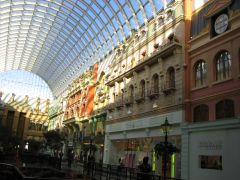
\includegraphics[width=.45\columnwidth]{Lorem}} \quad
\subfloat[Pan ma signo]
{\label{fig:example-b}%
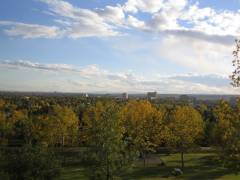
\includegraphics[width=.45\columnwidth]{Ipsum}} \\
\subfloat[Methodicamente o uno]
{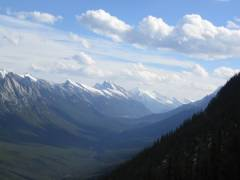
\includegraphics[width=.45\columnwidth]{Dolor}} \quad
\subfloat[Titulo debitas]
{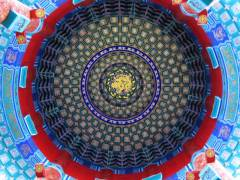
\includegraphics[width=.45\columnwidth]{Sit}}
\caption[Tu duo titulo debitas latente]{Tu duo titulo debitas latente}
\label{fig:example}
\end{figure}

Please note that the content of this section is just some dummy text. It isn't a real language.

Lorem ipsum dolor sit amet, consectetuer adipiscing elit. Ut purus elit, vestibulum ut, placerat ac, adipiscing vitae, felis. Curabitur dictum gravida mauris.

\subsection*{A subsection}

\lipsum[2]

\subsubsection*{A sub-subsection}

\lipsum[7]

\paragraph{A paragraph}
Lorem ipsum dolor sit amet, consectetuer adipiscing elit. Ut purus elit, vestibulum ut, placerat ac, adipiscing vitae, felis. Curabitur dictum gravida mauris. Nam arcu libero, nonummy eget, consectetuer id, vulputate a, magna.

\paragraph{Another paragraph}
Cras nec ante, pellentesque a nulla, cum sociis natoque penatibus et magnis dis parturient montes, nascetur ridiculus mus. Aliquam tincidunt urna

\bigskip

Donec aliquet, tortor sed accumsan bibendum, erat ligula aliquet magna, vitae ornare odio metus a mi. Morbi ac orci et nisl hendrerit mollis. Suspendisse ut massa. Cras nec ante. Pellentesque a nulla. Cum sociis natoque penatibus et magnis dis parturient montes, nascetur ridiculus mus. Aliquam tincidunt urna.

\begin{description}
\item[Mane] Lorem ipsum dolor sit amet, consectetuer adipiscing elit. 
\item[Tekel] Ut purus elit, vestibulum ut, placerat ac, adipiscing vitae, felis. Curabitur dictum gravida mauris.
\item[Fares] Nam arcu libero, nonummy eget, consectetuer 
id, vulputate a, magna.
\end{description}

\begin{table}
\caption{Lorem ipsum dolor sit amet}
\centering
\begin{tabular}{ll}
\toprule
\textbf{Alkaloid} & \textbf{Origin} \\
\midrule
atropine & belladonna \\
morphine & poppy \\
nicotine & tobacco \\
\bottomrule
\end{tabular}
\end{table}

Suspendisse vel felis. Ut lorem lorem, interdum eu, tincidunt sit amet, laoreet vitae, arcu. Aenean faucibus pede eu ante. Praesent enim elit, rutrum at, molestie non, nonummy vel, nisl. Ut lectus eros, malesuada sit amet, fermentum eu, sodales cursus, magna. Donec eu purus. Quisque vehicula, urna sed ultricies auctor, pede lorem egestas dui, et convallis elit erat sed nulla.

\subsection*{Some formulas}

Una formula in linea viene incorporata nel testo: $\lim_{n \to \infty}\sum_{k=1}^n \frac{1}{k^2} = \frac{\pi^2}{6}$, per esempio. Come si osserva, \LaTeX{} fa \emph{il possibile} per comprimerla e modificare il meno possibile l'interlinea nel capoverso che la contiene.
Una formula in display viene invece composta da \LaTeX{} su linee a parte, separate dal contesto con adeguati spazi bianchi per metterla in mostra e farla risaltare sulla pagina.
\begin{equation}
\lim_{n \to \infty}\sum_{k=1}^n \frac{1}{k^2}= \frac{\pi^2}{6}
\end{equation}
Come si osserva, ora la formula risulta centrata, non compressa, e tutti i suoi elementi occupano il giusto spazio con un risultato finale di grande respiro.

Integer tempus convallis augue. Etiam facilisis. Nunc elementum fermentum wisi. Aenean placerat. Ut imperdiet, enim sed gravida sollicitudin, felis odio placerat quam, ac pulvinar elit purus eget enim. 

\begin{equation}
\int_a^{a+T}f(x)\,dx= \int_0^T f(x)\,dx 
\qquad
\oint f(z)\,dz=2\pi i
\end{equation}

Nulla malesuada porttitor diam. Donec felis erat, congue non, volutpat at, tincidunt tristique, libero. Vivamus viverra fermentum felis. Donec non- ummy pellentesque ante.

\begin{equation}
f(x_1,\dots,x_n)=  \prod_{k=1}^n x_k 
\qquad
\sum_{k=1}^n x_k^2=1
\qquad
\biggl(\sum_n x_n^2\biggr)^{1/2} 
\end{equation}

\lipsum[2]

\begin{equation}
\begin{bmatrix} 
a_{11} & \dots & a_{1n} \\ 
a_{21} & \dots & a_{2n} \\ 
\hdotsfor{3} \\ 
a_{n1} & \dots & a_{nn} 
\end{bmatrix}
\end{equation}

\lipsum[4]

\begin{equation}
\lim_{x\to 0}
\frac{\sin x}{x}=1 \qquad
\lim_{n\to +\infty}f_n=\delta
\end{equation}

Fusce mauris. Vestibulum luctus nibh at lectus. Sed bibendum, nulla a faucibus semper, leo velit ultricies tellus, ac venenatis arcu wisi vel nisl. Vestibulum diam.

\begin{equation}
n!=
\begin{cases} 
1       & \text{if $n=0$} \\ 
n(n-1)! & \text{if $n\ge 1$} 
\end{cases} 
\end{equation}

Ut lectus eros, malesuada sit amet, fermentum eu, sodales cursus, magna. Donec eu purus. Quisque vehicula, urna sed ultricies auctor, pede lorem egestas dui, et convallis elit erat sed nulla. Donec luctus. Curabitur et nunc. Aliquam dolor odio, commodo pretium, ultricies non, pharetra in, velit.

\begin{equation} 
x_G=
\frac{\displaystyle
      \sum_{i=1}^n m_ix_i}
{\displaystyle\sum_{i=1}^n m_i}
\end{equation}

\lipsum[6]

\begin{equation}
\kappa =\frac{\xi}{E_{\textrm{max}}}
\qquad
E_{\textup{max}} =\frac{2 m_{\textup{e}} \beta^2\gamma^2 }{1 +2\gamma m_{\textup{e}}/m_{\textrm{x}} + ( m_{\textup{e}}/m_{\textup{x}})^2}
\end{equation}

\lipsum[8]
% !TEX encoding = UTF-8
% !TEX TS-program = pdflatex
% !TEX root = ../Tesi.tex
% !TEX spellcheck = it-IT

%************************************************
\chapter{Ipsum}
\label{cap:ipsum}
%************************************************

\lipsum[1]

\section{Lorem}
\lipsum[2]

\section{Ipsum}
\lipsum[3]

\section{Dolor}
\lipsum[4-5]
\appendix
% !TEX encoding = UTF-8
% !TEX TS-program = pdflatex
% !TEX root = ../Articolo.tex
% !TEX spellcheck = it-IT

%************************************************
\section{Dolor}
\label{sec:dolor}
%************************************************

\lipsum[1]

\subsection{Mane}
\lipsum[2]

\subsection{Tekel}
\lipsum[3]

\subsection{Fares}
\lipsum[4-5]

% *****************************************************************
% Materiale finale
%******************************************************************
% !TEX encoding = UTF-8
% !TEX TS-program = pdflatex
% !TEX root = ../CME-III-ARTICOLO.tex
% !TEX spellcheck = it-IT

%*******************************************************
% Bibliografia
%*******************************************************
\nocite{*}
\printbibliography
% !TEX encoding = UTF-8
% !TEX TS-program = pdflatex
% !TEX root = ../Tesi.tex
% !TEX spellcheck = it-IT

%*******************************************************
% Dichiarazione
%*******************************************************
\cleardoublepage
\phantomsection
\pdfbookmark{Dichiarazione}{Dichiarazione}
\chapter*{Dichiarazione}
\thispagestyle{empty}

Lorem ipsum dolor sit amet, consectetuer adipiscing elit. Ut purus elit, vestibulum ut, placerat ac, adipiscing vitae, felis. Curabitur dictum gravida mauris. Nam arcu libero, nonummy eget, consectetuer id, vulputate a, magna. Donec vehicula augue eu neque.

Pellentesque habitant morbi tristique senectus et netus et malesuada fames ac turpis egestas. Mauris ut leo. Cras viverra metus rhoncus sem. Nulla et lectus vestibulum urna fringilla ultrices.

\bigskip
 
\noindent\textit{\myLocation, \MakeTextLowercase{\myTime}}

\smallskip

\begin{flushright}
    \begin{tabular}{m{5cm}}
        \\ \hline
        \centering\myName \\
    \end{tabular}
\end{flushright}

\end{document}